\chapter{Results}


\Large Here we present some results of the output from the Unity Engine that are  auto generate output using L system which is shown on figure \ref{fig:road}, Road generated with in less than 2 second as the whole path is calculated with rules of string and some of them are ignored to create more randomization.

\begin{figure}[h]
\caption{Example of a random generated road using L system}
\label{fig:road}
\vspace{0.3cm}
\centering
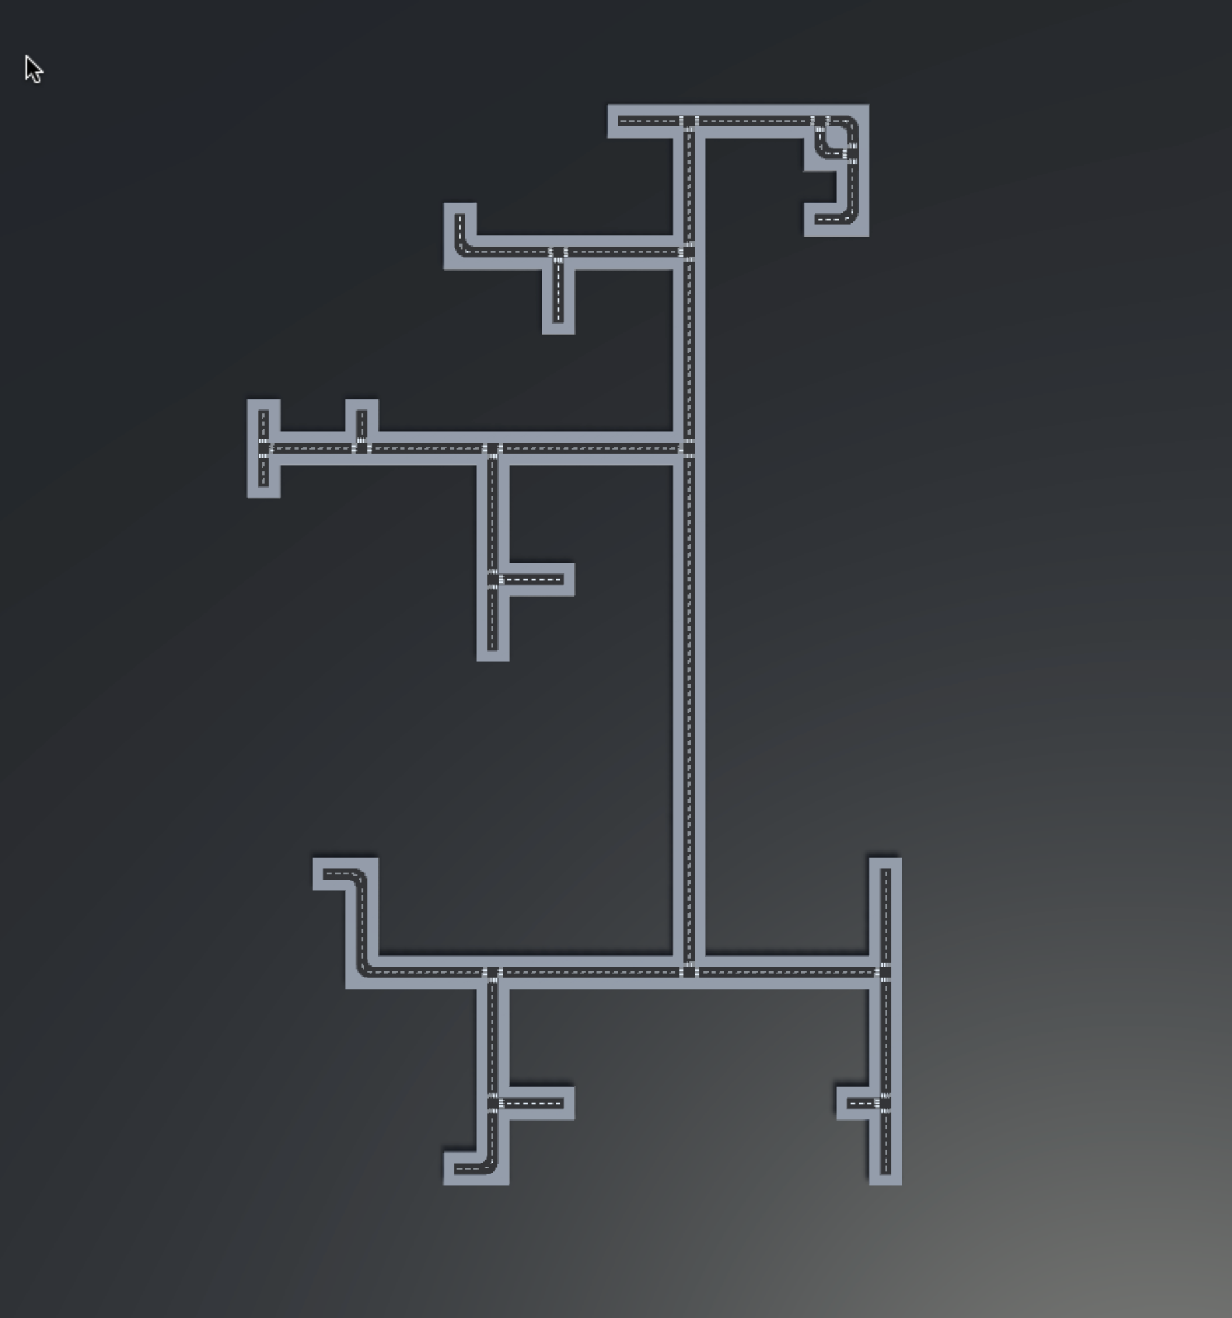
\includegraphics[width=0.6\textwidth]{5. results/Road Outpu.png}
\end{figure}

\renewcommand{\baselinestretch}{1.5}
\begin{scriptsize}
\begin{lstlisting} [language=C++, frame=single]
/// <summary>
/// Generates the string 
/// </summary>
/// <param name="newWord">Everything adds upto this word </param>
/// <param name="c">each character in the rule</param>
/// <param name="iterationIndex">number of iterations </param>
private void ProcessRulesRecursivelly(StringBuilder newWord, char c, int iterationIndex)
{
    foreach (var rule in rules)
    {
        if(rule.letter==c.ToString())
        {
            if (randomIgnoreRuleModifier)
            {
                if (Random.value < chanceToIgnoreRules && iterationIndex > 1)
                {
                    Debug.Log("Rule Ignored");
                    return;
                }
            }
            newWord.Append(GrowRecursive(rule.GetResult(), iterationIndex + 1));
        }
    }
}
\end{lstlisting}

\end{scriptsize}

\renewcommand{\baselinestretch}{1.5}

\Large Shown in figure \ref{fig:road} the models of road are textured before are brought in to the unity so they are placed based on the direction that adds up to the either side of the roads.

\vspace{0.5cm}

\Large House and tress are placed with respective to road layout the figure \ref{fig:city} shows the output after they generated with L system model. They are structured based on the rules of the constants of F as axiom and constants are [, ], +, - which are used to define the rule system.

\begin{figure}[h]
\caption{Example of a random generated city using L system}
\label{fig:city}
\vspace{0.3cm}
\centering
\includegraphics[width=0.8\textwidth]{5. results/City.png}
\end{figure}
